%\documentclass[10pt]{beamer}
\documentclass[10pt,aspectratio=169,usenames,dvipsnames]{beamer}

\usetheme[progressbar=frametitle]{metropolis}
\usepackage{appendixnumberbeamer}

\usepackage{booktabs}
\usepackage[scale=2]{ccicons}

\usepackage{pgfplots}
\usepgfplotslibrary{dateplot}

\usepackage{xspace}
\newcommand{\themename}{\textbf{\textsc{metropolis}}\xspace}

\usepackage{graphicx}

\setbeamertemplate{enumerate items}[circle]

\usepackage{pict2e}

\usepackage{media9}

\usepackage{amsmath}

\usepackage{mathtools}
\DeclarePairedDelimiter\abs{\lvert}{\rvert}%
\DeclarePairedDelimiter\norm{\lVert}{\rVert}%
\makeatletter
\let\oldabs\abs
\def\abs{\@ifstar{\oldabs}{\oldabs*}}

\usepackage[makeroom]{cancel}

\usepackage{xcolor}
\usepackage{soul}
\newcommand{\mathcolorbox}[2]{\colorbox{#1}{$\displaystyle #2$}}

\title{Stoke Theorem: connecting surface and line integrals}
%ABSTRACT: 
\date{}
\author{\textbf{\textcolor{black}{Ben Snow}}}
\institute{\textcolor{black}{University of Exeter} \\ \textcolor{black}{St Andrews, 17th March 2023.}}


%\titlegraphic{\vspace{-0.7cm} \hspace{-1.3cm}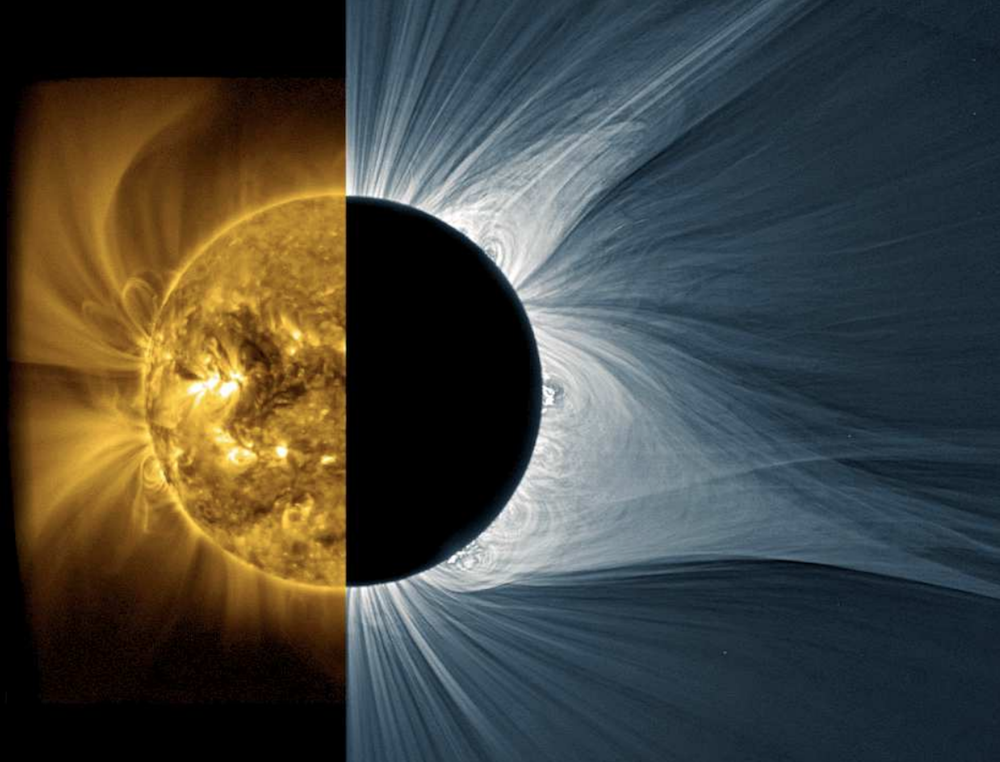
\includegraphics[width=\paperwidth,height=\paperheight]{2023Dundee/Figures/SolarCoronaDouble.png}}

\begin{document}

\maketitle

\begin{frame}{Recap - line integral}
\begin{columns}
\begin{column}{0.5\textwidth}
Arbitrary integral over a continuous curve
\begin{gather}
    \int_C \textbf{F} \cdot \,d\textbf{r}
\end{gather}
where $\textbf{F}$ is an arbitrary vector, $C$ is the line/path to integrate over, $d\textbf{r}$ is small step along a curve.\\
Note that in this lesson, $C$ will be a \textbf{closed} path.
\end{column}
\begin{column}{0.5\textwidth}
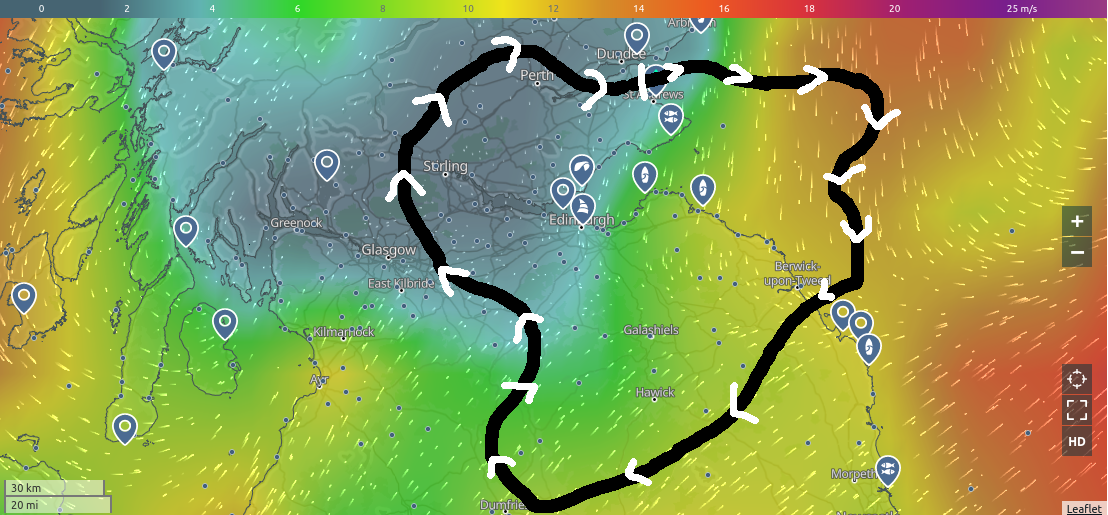
\includegraphics[width=0.95\linewidth]{2023StAndrews/lineexample.png} \\
Suppose a bird is travelling around Scotland on the path shown. It is subject to a force from the wind. The line integral can tell us if this force was generally helpful or not.
%\includegraphics[width=0.32\linewidth]{Figures/Crab_Nebula.jpeg}
%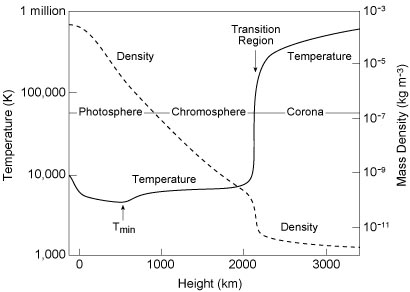
\includegraphics[width=0.95\linewidth]{2023Dundee/Figures/valc.png} \\
%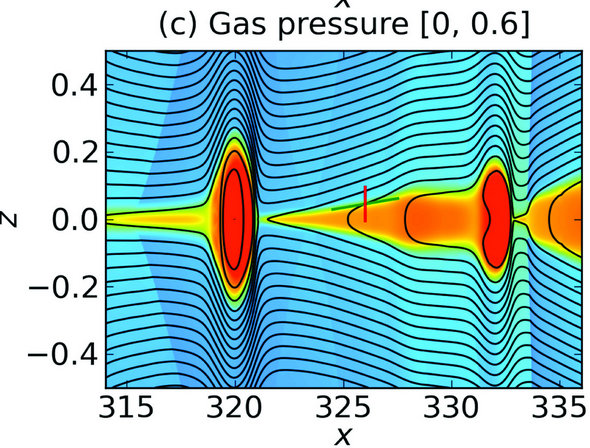
\includegraphics[width=0.95\linewidth]{2023RAS/Figures/shibyama.png}
%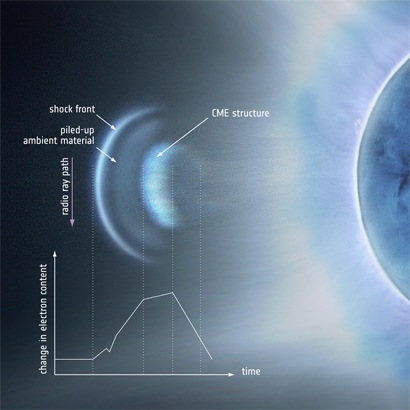
\includegraphics[width=0.32\linewidth]{Figures/cmesketch.jpg}
\end{column}
\end{columns}
\end{frame}

\begin{frame}{Recap - surface integral}
\begin{columns}
\begin{column}{0.5\textwidth}
Arbitrary integral over an arbitrary surface
\begin{gather}
    \iint_S \textbf{F} \cdot \,d\textbf{S}
\end{gather}
where $\textbf{F}$ is an arbitrary vector, $S$ is the surface over which to integrate, $d\textbf{S}$ is small step along a surface.
\end{column}
\begin{column}{0.5\textwidth}
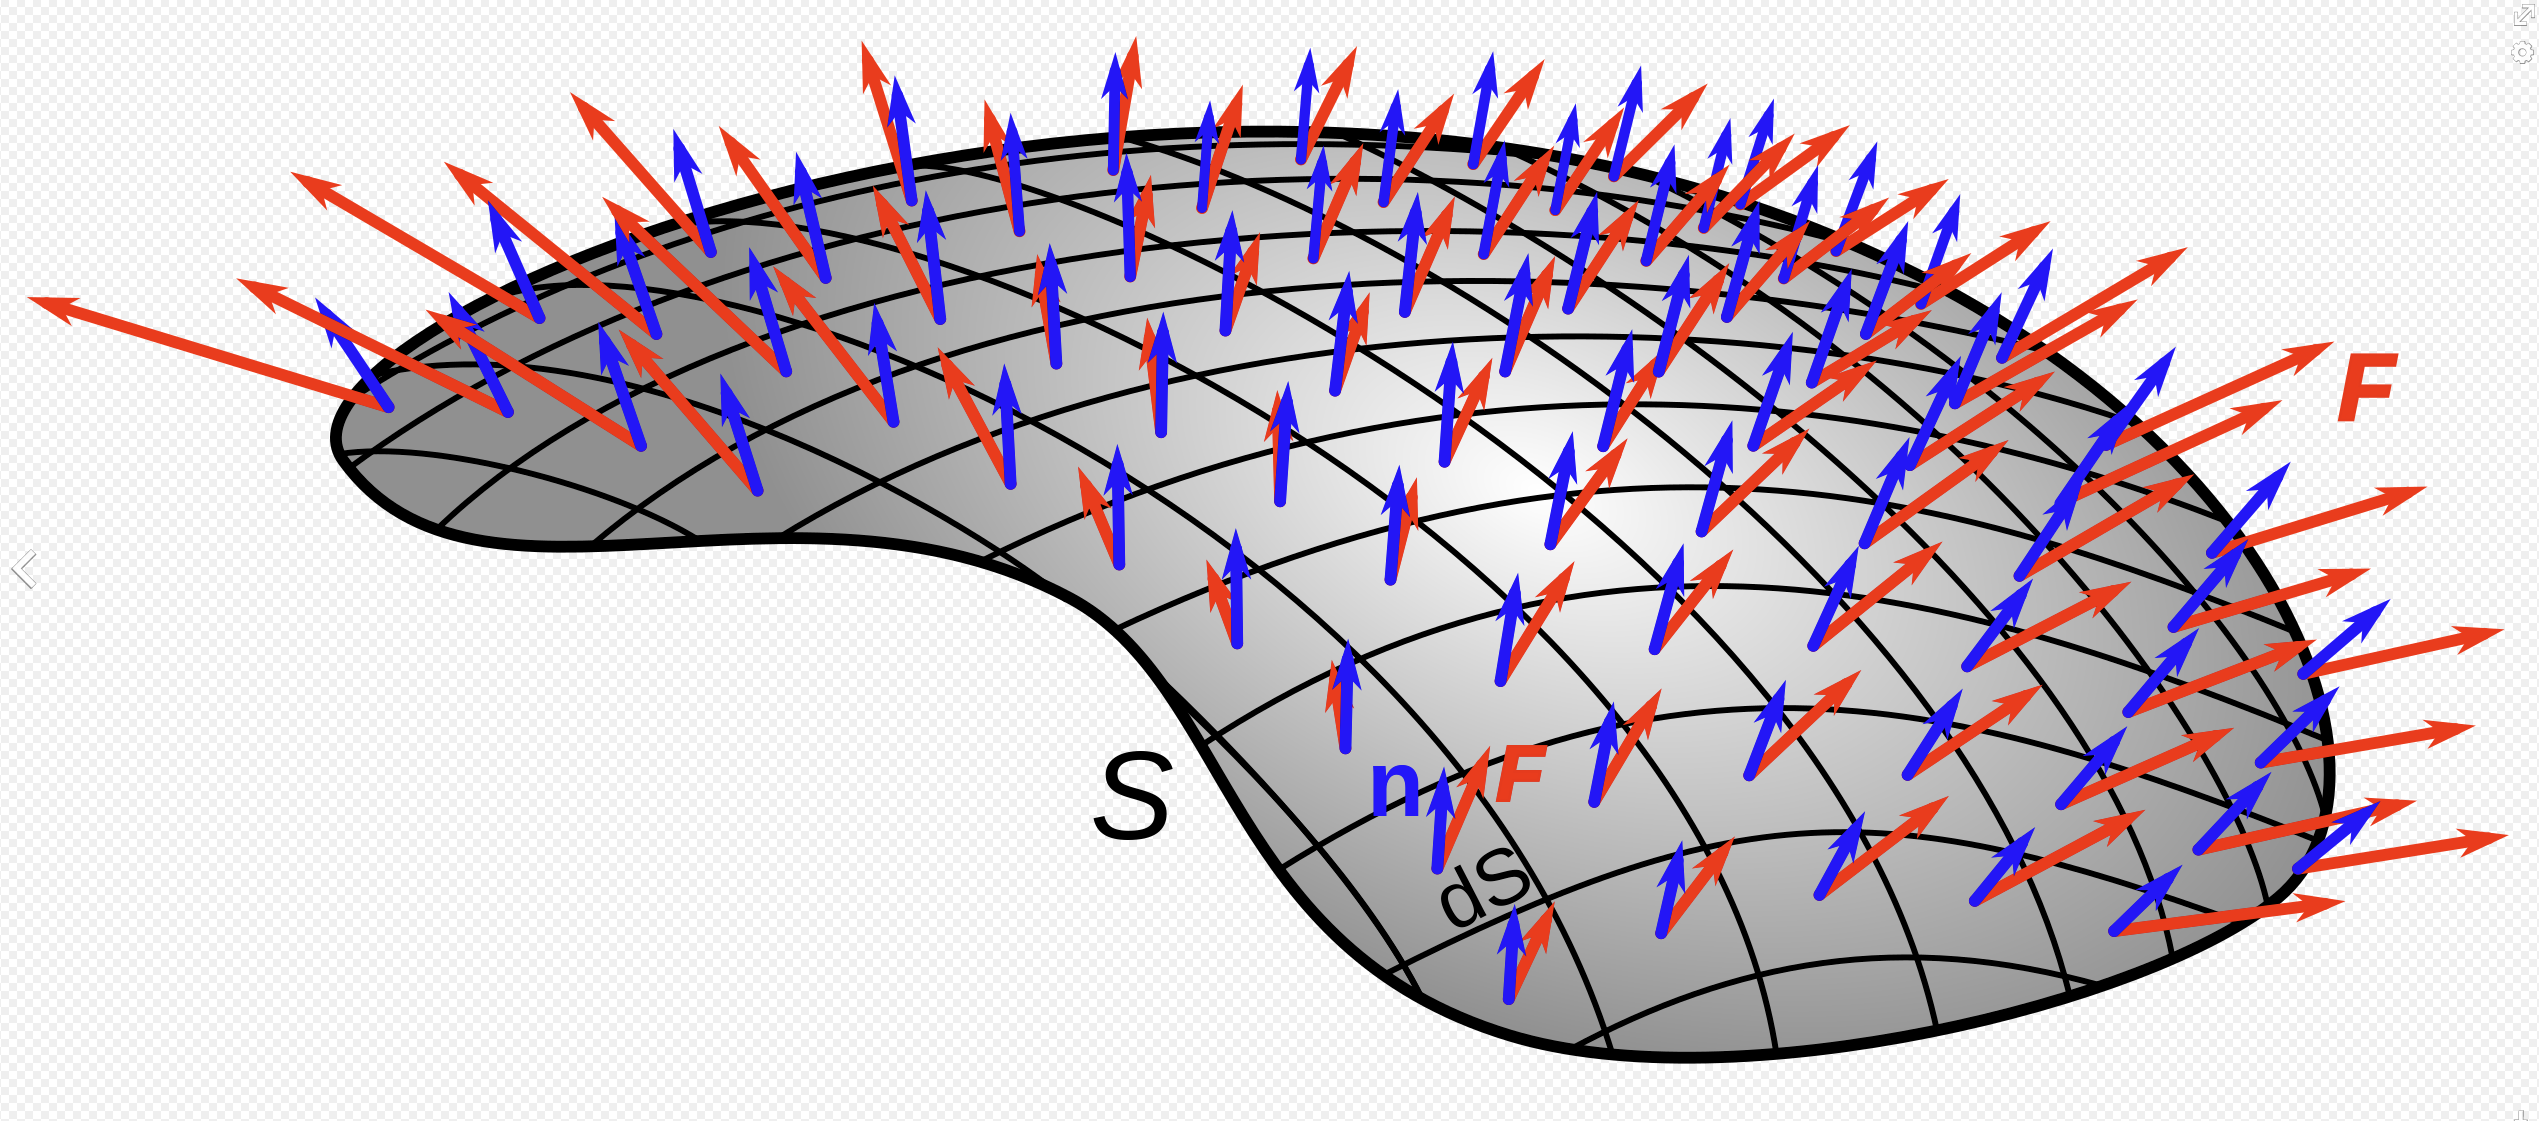
\includegraphics[width=0.8\linewidth]{2023StAndrews/Screenshot from 2023-03-13 14-36-16.png} \\
Break up a surface into arbitrarily small section $dS$. Flux through surface is the sum of the force normal to the section ($\textbf{F}\cdot \textbf{n} dS$).
% Suppose a bird is travelling around Scotland on the path shown. It is subject to a force from the wind. The line integral can tell us if this force was generally helpful or not.
%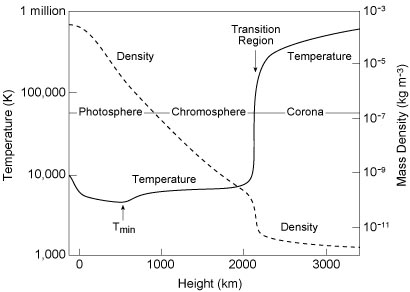
\includegraphics[width=0.95\linewidth]{2023Dundee/Figures/valc.png} \\
%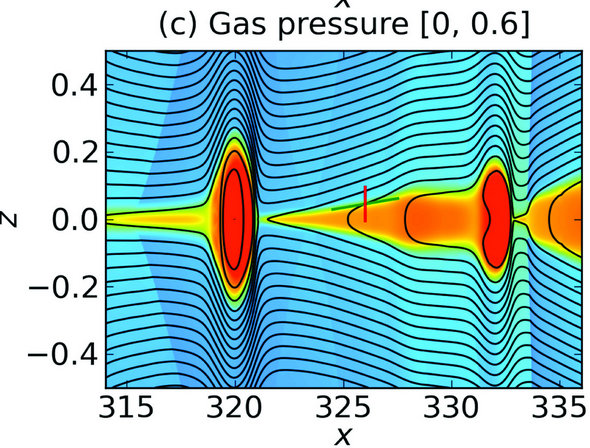
\includegraphics[width=0.95\linewidth]{2023RAS/Figures/shibyama.png}
%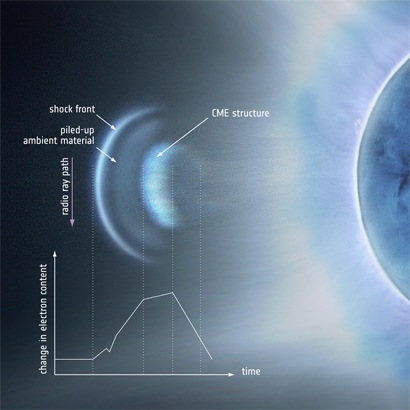
\includegraphics[width=0.32\linewidth]{Figures/cmesketch.jpg}
\end{column}
\end{columns}
\end{frame}

\begin{frame}{Stokes Theorem}
Connects line integrals to surface integrals according to
\begin{gather}
    \int_C \textbf{F} \cdot \,d\textbf{r} = \iint_S \nabla \times \textbf{F} \,d\textbf{S}
\end{gather}
where $\nabla \times \textbf{F}$ is the curl (or rot) of $F$.

\textbf{The line integral of a vector field over a loop is equal to the flux of its curl through the enclosed surface.}
\end{frame}

%%%%%%%%%%%%%%%%%%%%%%%%%%%%%%%%%%%%%%%%%%%%%%%%%%%%%%%%%%%%%%%%%%%%%%%%%%%%%%%%%%%%%%%%%
\begin{frame}{Stokes Theorem - proof}
\begin{columns}
\begin{column}{0.5\textwidth}
\begin{itemize}
    \item Define an arbitrary surface
    \item A surface has a closed loop aound its boundary
    \item Line integral along closed loop defined as:
\end{itemize}
\begin{gather}
    \int_C \textbf{F} \cdot \,d\textbf{r}
\end{gather}
\end{column}
\begin{column}{0.5\textwidth}
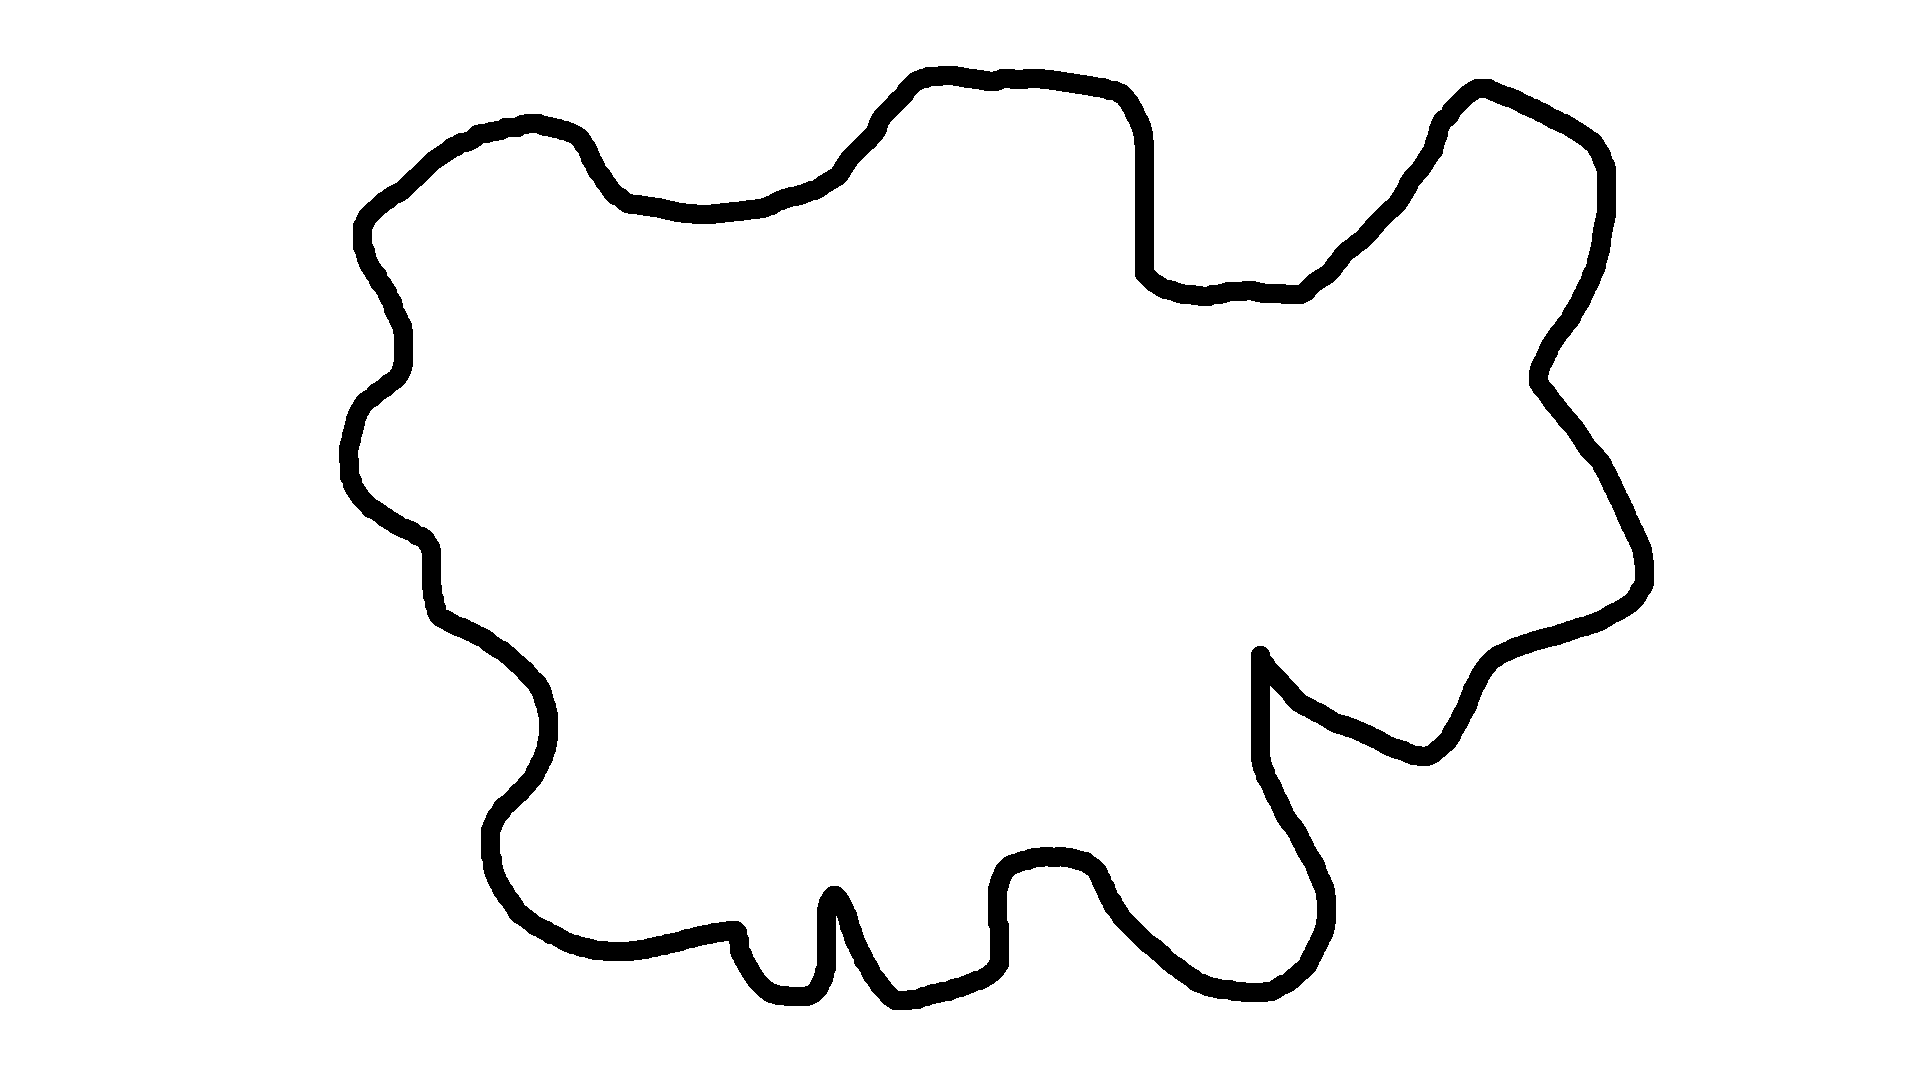
\includegraphics[width=0.8\linewidth]{2023StAndrews/surface.png}
\end{column}
\end{columns}
\end{frame}

\begin{frame}{Stokes Theorem - proof}
\begin{columns}
\begin{column}{0.5\textwidth}
\begin{itemize}
    \item Split surface into two pieces
    \item Keep direction the same!
    \item Line integral along each piece equals line integral over whole surface:
\end{itemize}
\begin{gather}
    \int_{C1} \textbf{F} \cdot \,d\textbf{r}+\int_{C2} \textbf{F} \cdot \,d\textbf{r}=\int_C \textbf{F} \cdot \,d\textbf{r}
\end{gather}
\end{column}
\begin{column}{0.5\textwidth}
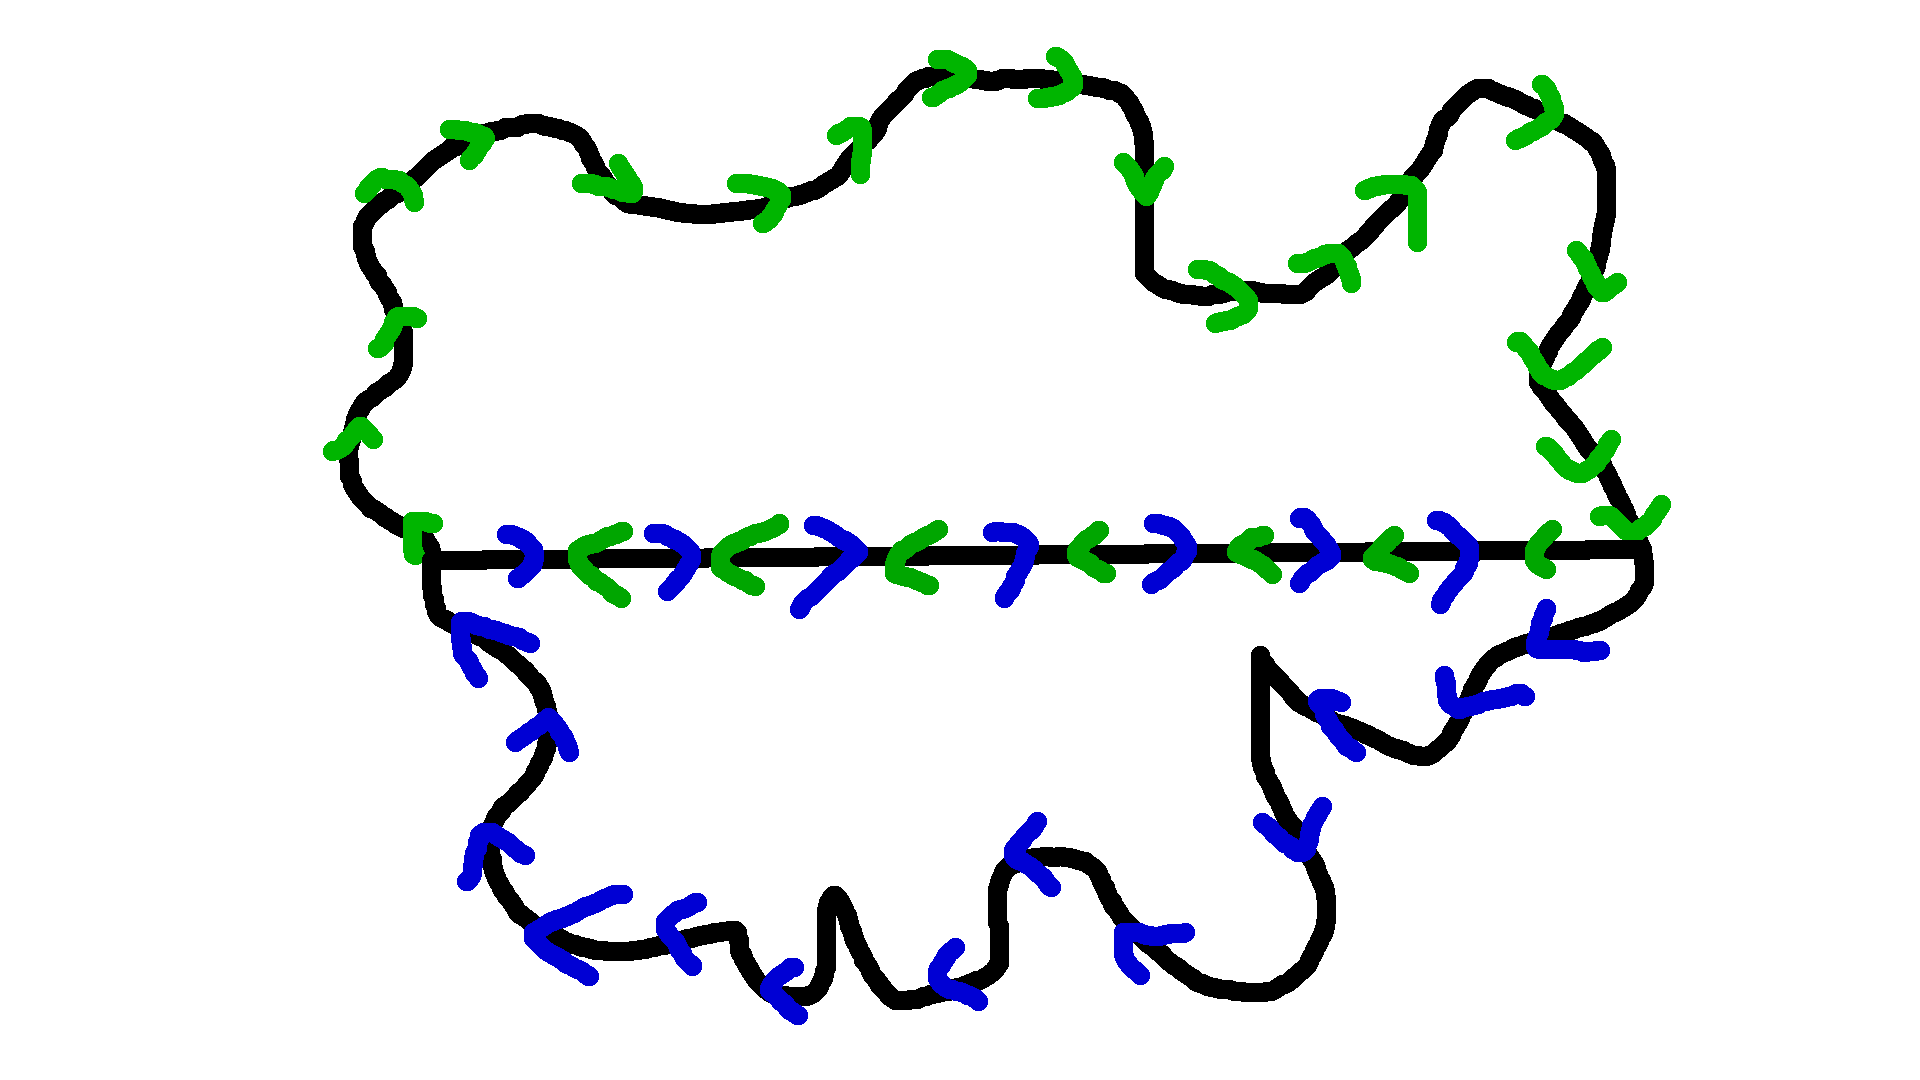
\includegraphics[width=0.8\linewidth]{2023StAndrews/surface2.png}
\end{column}
\end{columns}
\end{frame}

\begin{frame}{Stokes Theorem - proof}
\begin{columns}
\begin{column}{0.5\textwidth}
\begin{itemize}
    \item Break into infinitely small sections
    \item Line integral over surface $C_k$ gives rotation on surface
    \item Rotation also calculable using curl operator
\end{itemize}
\begin{gather}
    \int_{Ck} \textbf{F} \cdot \,d\textbf{r} \approx \left( \nabla \times \textbf{F}(x_k,y_k,z_k) \right) \cdot \hat{n} \,dS
\end{gather}
\end{column}
\begin{column}{0.5\textwidth}
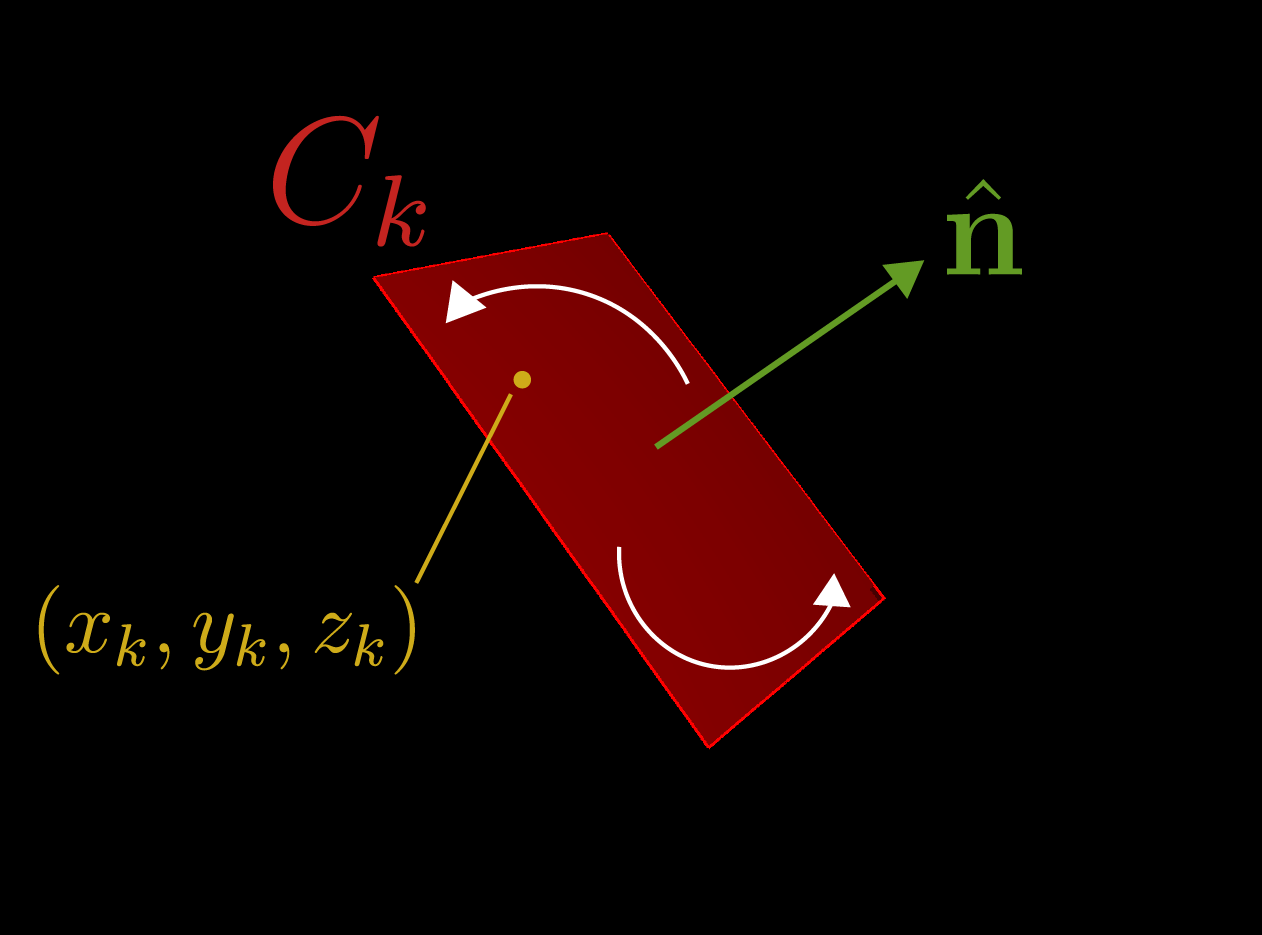
\includegraphics[width=0.8\linewidth]{2023StAndrews/ds.png}
\end{column}
\end{columns}
\end{frame}

\begin{frame}{Stokes Theorem - proof}
\begin{itemize}
    \item Sum of all infinitely small sections gives line integral over the loop
\end{itemize}
\begin{gather}
    \sum_{k=1}^{n} \int_{Ck} \textbf{F} \cdot \,d\textbf{r} \approx \sum_{k=1}^{n}  \left( \nabla \times \textbf{F}(x_k,y_k,z_k) \right) \cdot \hat{n} \,dS
\end{gather}
\begin{itemize}
    \item As $d\textbf{r},d\textbf{S} \xrightarrow{} 0$, the sumation approaches the true integral, therefore,
\end{itemize}
\begin{gather}
    \int_C \textbf{F} \cdot \,d\textbf{r} = \iint_S \nabla \times \textbf{F} \,d\textbf{S}
\end{gather}
\textbf{The line integral of a vector field over a loop is equal to the flux of its curl through the enclosed surface.}
\end{frame}

%%%%%%%%%%%%%%%%%%%%%%%%%%%%%%%%%%%%%%%%%%%%%%%%%%%%%%%%%%%%%%%%%%%%%%%%%%%%%%%%%%%%%%%%%
\begin{frame}{Stokes Theorem}
\begin{columns}
\begin{column}{0.5\textwidth}
\begin{itemize}
    \item Requires a closed loop for the line integral
    \item 2D equivalent is the Greene's Theorem:  the macroscopic circulation around the curve C equals the sum of all the microscopic circulation that is inside C
    \item Further reading: Stewart, James (2012). Calculus - Early Transcendentals (7th ed.). Brooks/Cole Cengage Learning. p. 1122
\end{itemize}
\end{column}
\begin{column}{0.5\textwidth}
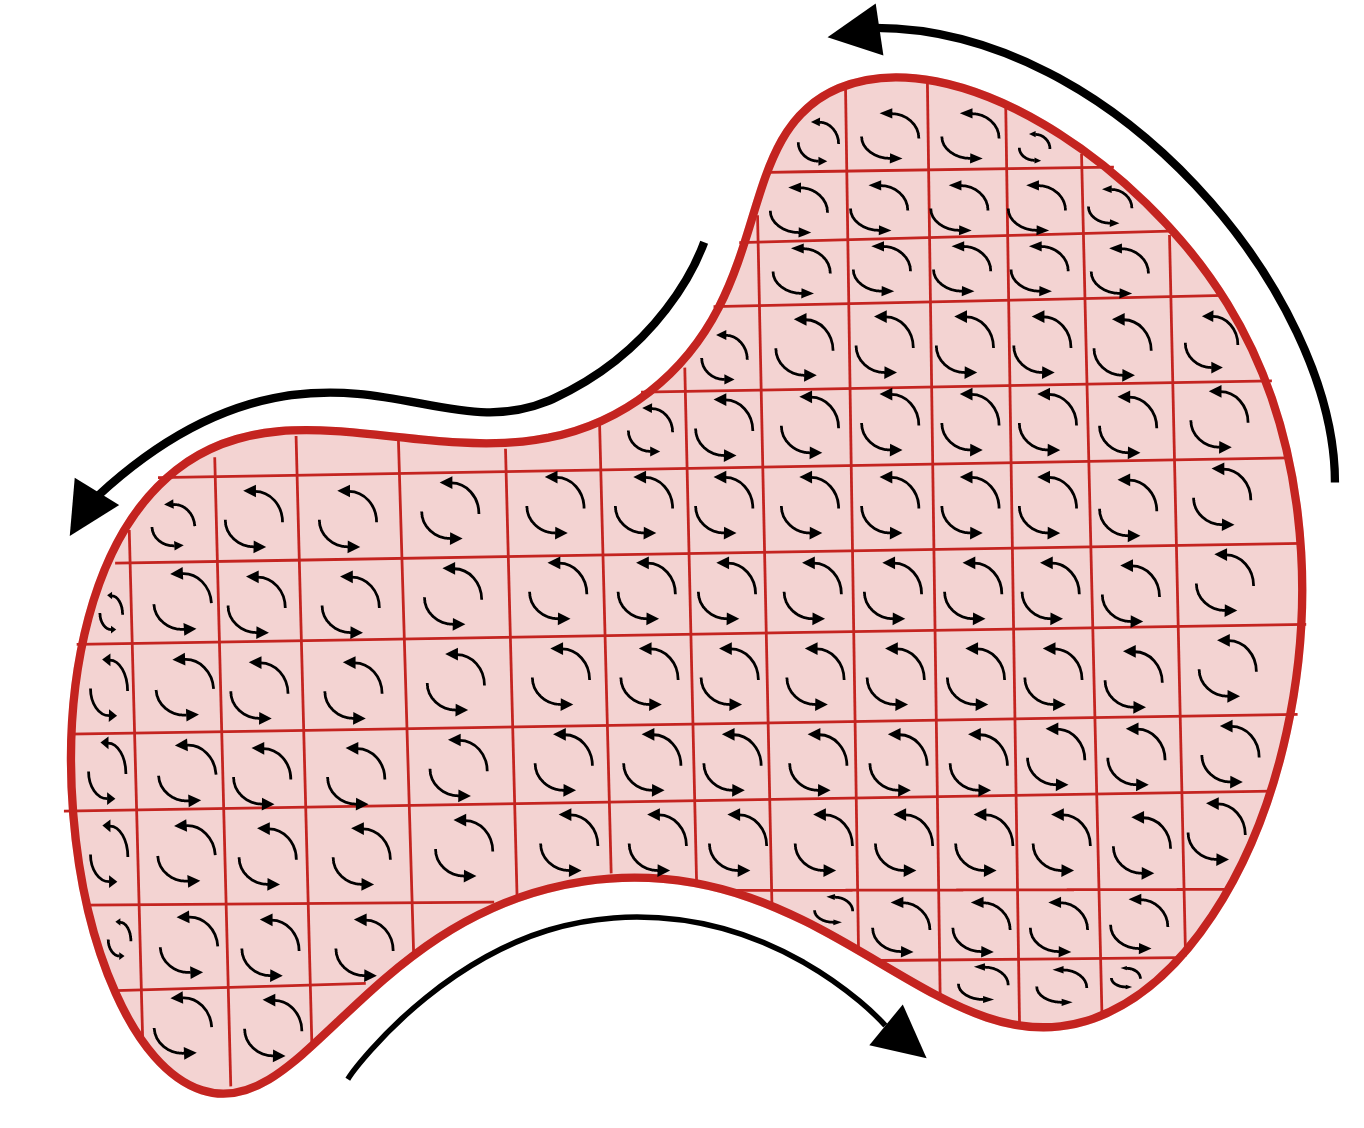
\includegraphics[width=0.8\linewidth]{2023StAndrews/Screenshot from 2023-03-15 06-49-01.png}
\end{column}
\end{columns}
\end{frame}

\end{document}
